\documentclass{report}
\usepackage[a4paper, margin=0.5in]{geometry}
\usepackage{parskip}
\usepackage{graphicx}
\usepackage{caption}
\usepackage{amssymb}
\usepackage{amsmath}
\usepackage{algpseudocode}
\usepackage{algorithm}

\captionsetup[figure]{
  font = it,
  labelfont = bf
}

\begin{document}
\begin{minipage}[b]{0.48\textwidth}
  \section*{K-Means Clustering}
  A clustering algorithm is an algorithm designed with the purpose of grouping, into an arbitrary number of classes, a set of points. Such classes are created by trying to group together points that have common features. Thus, the goal of this category of algorithms is to build knowledge about the data provided as input that makes it possible to find hidden relationships among the data, or to classify (into one of the classes created in the training stages) a point whose class is not known a priori.

  \section*{Standard (or Lloyd) Algorithm}
  In this section, the standard algorithm for implementing k-means clustering is introduced. 

  First, it is important to define the initial condition (i.e., the input data) on which the algorithm will be run. Considering the case in two dimensions, the input is a collection of points that are randomly placed in 2D space (Figure \ref{fig:rndpoints}).

  \begin{center} 
      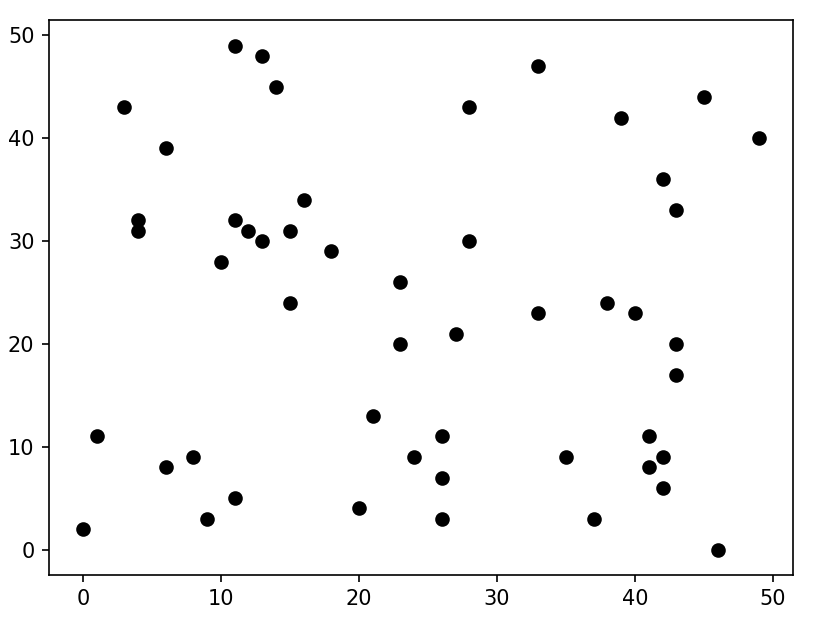
\includegraphics[width = 0.9\textwidth]{imgs/rndpoints.png}
      \captionof{figure}{Initial distribution of random points}
      \label{fig:rndpoints}
  \end{center}

  The first step is to generate an arbitrary number of \textbf{centroids}, i.e., points in space representing the classes to which points will be assigned according to a criterion of maximum closeness.

  \begin{center}
      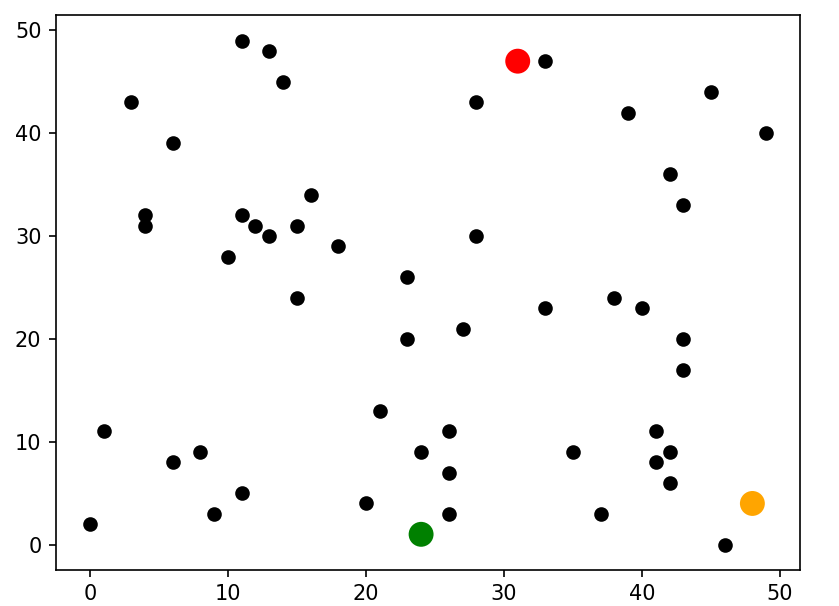
\includegraphics[width = 0.9\textwidth]{imgs/rndcens.png}
      \captionof{figure}{ Random initial position of centroids }
      \label{fig:rndcens}
  \end{center}

  Figure \ref{fig:rndcens} shows three centroids representing 3 classes (red, green, orange). The generation of centroids can be done in 2 ways: by choosing as centroids some of the points provided as input, or by randomly generating them in space.

  After that the centroids are generated, each point is assigned a class according to the principle of maximum closeness. 

\end{minipage}
\hspace{0.1in}
\begin{minipage}[b]{0.48\textwidth}
  That is, given a point P = (x, y) in space its membership class is the class represented by the centroid whose distance from the point is less than that of all other centroids. The choice of how to measure the distance between two points in space affects the final result of the classification. Therefore it is necessary to specify which measure is being used, in this case the \textbf{Euclidean distance}. Given two points A = ($a_x$, $a_y$) and B = ($b_x$, $b_y$) the Euclidean distance is calculated as
  \begin{equation}
      d(A, B) = \sqrt{(a_x - b_x)^2 + (a_y - b_y)^2}
  \end{equation}

  Figure \ref{fig:pointasgn} shows the application of the above to assign a class to each point.

  \begin{center}    
      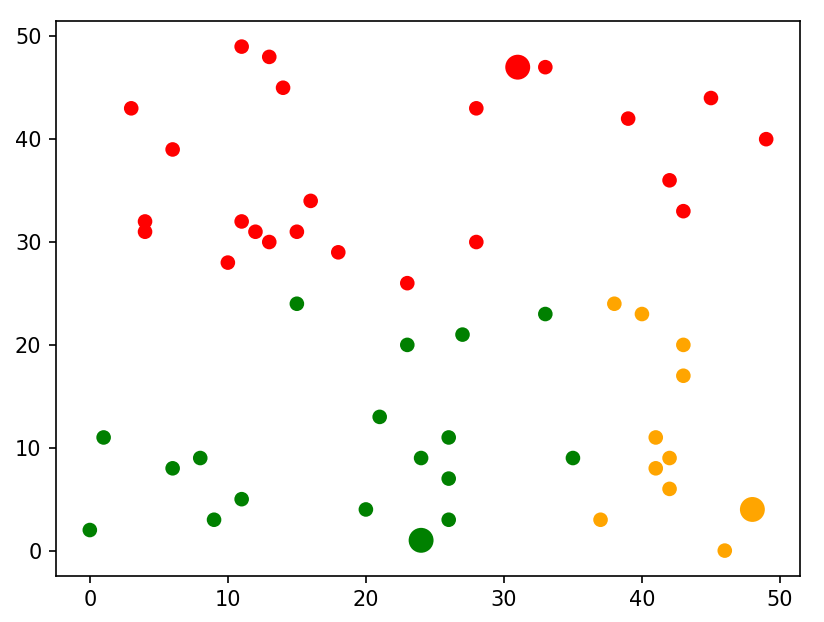
\includegraphics[width = 0.9\textwidth]{imgs/asgnpoints.png}
      \captionof{figure}{Punti dopo l'assegnazione delle classi}
      \label{fig:pointasgn}
  \end{center}

  The next step is to reposition the centroids by calculating the average of all points belonging to its class. If $C_i = (C_i^x, C_i^y)$ is the i-th centroid, its new position ($\tilde{C_i}$) can be calculated as
  \begin{equation}
      \tilde{C_i^x} = \frac{1}{N_i}\cdot \sum_{j = 1}^{N_i} P_{ij}^x
  \end{equation}
  \begin{equation}
      \tilde{C_i^y} = \frac{1}{N_i}\cdot \sum_{j = 1}^{N_i} P_{ij}^y
  \end{equation}

  Dove $N_i$ è il numero di punti appartenenti all'i-esima classe e $P_{ij}$ è il j-esimo punto appartenente all'i-esima classe. 

  La Figura \ref{fig:reccens} mostra i centroidi dopo essere stati riposizionati. 
  
  \begin{center}    
      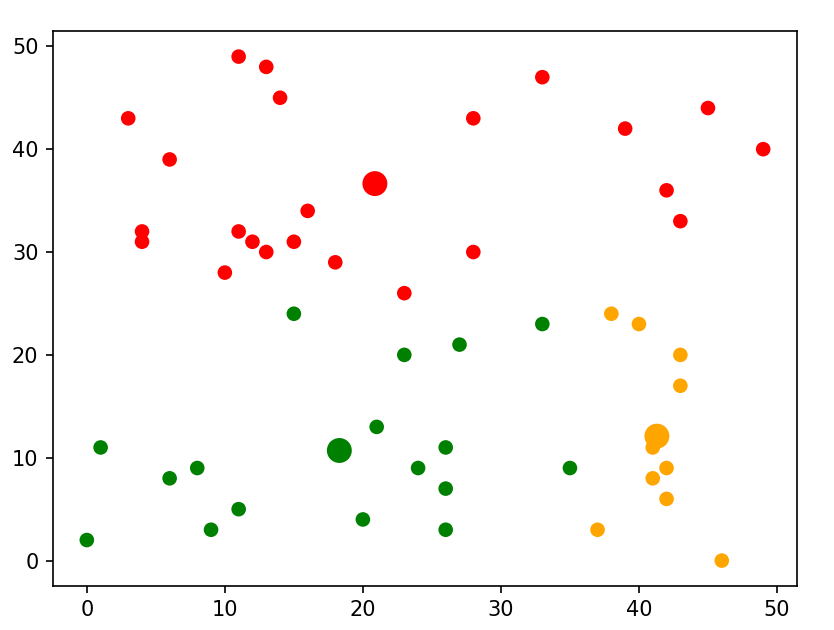
\includegraphics[width = 0.9\textwidth]{imgs/reccens.png}
      \captionof{figure}{Punti dopo l'assegnazione delle classi}
      \label{fig:reccens}
  \end{center}

  At this point, the steps seen so far are repeated, that is, classes are reassigned to the points and the centroids are shifted 
\end{minipage}

\newpage

\begin{minipage}[b]{0.48\textwidth}
  until a convergence criterion is reached, which for example could be when the centroids do not shift more than a certain threshold, or simply after a certain number of iterations. This latter method could be usefull when comparing two different algorithm (like lloyd vs hamerly algorithm which is described later)  because the two could converge after a different number of iterations therefore by using a fixed number of repetitions it is easy to compare the result after the same number of cycles. Because of this, for this report, the second approach has been used.

  \section*{Number of iterations}
  The iterations required during a single cycle are \[N\cdot K\cdot d\] where $N$ is the number of points, $K$ is the number of centroids and k is the dimensionality of the data. This is because for each point it is necessary to calculate the distance to each centroid to know which is the least, and to calculate the distance it is necessary to sum k terms (one for each dimension).

  So if m is the number of cycles, the iterations needed are in total
  \begin{equation}
    m(N\cdot K\cdot d)
  \end{equation}

  \begin{algorithm}[H]
    \caption{k-means pseudo-code}\label{alg:cap}
    \begin{algorithmic}
        \State Let P be the set of all points $P_i$
        \State Let C be the set of all centroids $C_i$
        \For{ l $<$ iterations }
        \\
        \Comment Point assignation
        \For{ $P_i$ in P }
            \State $d_{min}$ = d($C_1$, $P_i$)
            \State classe = $C_1$
            \For{$C_{j\neq 1}$ in C}
                \State d = d($C_j$, $P_i$)
                \If{d < $d_{min}$}
                    \State $d_{min} = d$
                    \State classe = $C_j$
                \EndIf
            \EndFor
        \EndFor
        \\
        \Comment Centroid update
        \State Let $P_{Ci}$ be the set of points with class $C_i$
        \For {$C_i$ in C}
            \State $\tilde{C_i}^x$ = 0
            \State $\tilde{C_i}^y$ = 0

            \For{p in $P_{Ci}$}
                \State  $\tilde{C_i}^x = \tilde{C_i}^x + p^x$
                \State  $\tilde{C_i}^y = \tilde{C_i}^y + p^y$
            \EndFor

            \State $C_i^x = \tilde{C_i}^x/size(P_{Ci})$
            \State $C_i^y = \tilde{C_i}^y/size(P_{Ci})$
        \EndFor
      \EndFor
    \end{algorithmic}
\end{algorithm}
\end{minipage}
\hspace{0.1in}
\begin{minipage}[b]{0.48\textwidth}

\end{minipage}

\end{document}